\documentclass[paper=letter,11pt]{scrartcl}

\KOMAoptions{headinclude=true, footinclude=false}
\KOMAoptions{DIV=14, BCOR=5mm}
\KOMAoptions{numbers=noendperiod}
\KOMAoptions{parskip=half}
\addtokomafont{disposition}{\rmfamily}
\addtokomafont{part}{\LARGE}
\addtokomafont{descriptionlabel}{\rmfamily}
%\setkomafont{pageheadfoot}{\normalsize\sffamily}
\setkomafont{pagehead}{\normalsize\rmfamily}
%\setkomafont{publishers}{\normalsize\rmfamily}
\setkomafont{caption}{\normalfont\small}
\setcapindent{0pt}
\deffootnote[1em]{1em}{1em}{\textsuperscript{\thefootnotemark}\ }


\usepackage{amsmath}
\usepackage[varg]{txfonts}
\usepackage[T1]{fontenc}
\usepackage{graphicx}
\usepackage{xcolor}
\usepackage[american]{babel}
% hyperref is needed in many places, so include it here
\usepackage{hyperref}

\usepackage{xspace}
\usepackage{multirow}
\usepackage{float}


\usepackage{braket}
\usepackage{bbm}
\usepackage{relsize}
\usepackage{tcolorbox}


\def\x{\ensuremath{x}}
\def\xp{\ensuremath{x'}}
\def\t{\ensuremath{t}}
\def\tp{\ensuremath{t'}}
\def\v{\ensuremath{v}}
%\def\nus{$\nu$s}

%\def\ketY{\ensuremath{\ket {\Psi}}}
%\def\iGeV{\ensuremath{\textrm{GeV}^{-1}}}
%%\def\mp{\ensuremath{m_{\textrm{proton}}}}
%\def\rp{\ensuremath{r_{\textrm{proton}}}}
%\def\me{\ensuremath{m_{\textrm{electron}}}}
%\def\aG{\ensuremath{\alpha_G}}
%\def\rAtom{\ensuremath{r_{\textrm{atom}}}}
%\def\rNucl{\ensuremath{r_{\textrm{nucleus}}}}
%\def\GN{\ensuremath{\textrm{G}_\textrm{N}}}
%\def\ketX{\ensuremath{\ket{\vec{x}}}}
%\def\ve{\ensuremath{\vec{\epsilon}}}
%
%
%\def\ABCDMatrix{\ensuremath{\begin{pmatrix} A &  B  \\ C  & D \end{pmatrix}}}
%\def\xyprime{\ensuremath{\begin{pmatrix} x' \\ y' \end{pmatrix}}}
%\def\xyprimeT{\ensuremath{\begin{pmatrix} x' &  y' \end{pmatrix}}}
%\def\xy{\ensuremath{\begin{pmatrix} x \\ y \end{pmatrix}}}
%\def\xyT{\ensuremath{\begin{pmatrix} x & y \end{pmatrix}}}
%
%\def\IMatrix{\ensuremath{\begin{pmatrix} 0 &  1  \\ -1  & 0 \end{pmatrix}}}
%\def\IBoostMatrix{\ensuremath{\begin{pmatrix} 0 &  1  \\ 1  & 0 \end{pmatrix}}}
%\def\JThree{\ensuremath{\begin{pmatrix}    0 & -i & 0  \\ i & 0  & 0 \\ 0 & 0 & 0 \end{pmatrix}}} 
%\def\JTwo{\ensuremath{\begin{bmatrix}    0 & 0 & -i  \\ 0 & 0  & 0 \\ i & 0 & 0 \end{bmatrix}}}
%\def\JOne{\ensuremath{\begin{bmatrix}    0 & 0 & 0  \\ 0 & 0  & -i \\ 0 & i & 0 \end{bmatrix}}}
%\def\etamn{\ensuremath{\eta_{\mu\nu}}}
%\def\Lmn{\ensuremath{\Lambda^\mu_\nu}}
%\def\dmn{\ensuremath{\delta^\mu_\nu}}
%\def\wmn{\ensuremath{\omega^\mu_\nu}}
%\def\be{\begin{equation*}}
%\def\ee{\end{equation*}}
%\def\bea{\begin{eqnarray*}}
%\def\eea{\end{eqnarray*}}
%\def\bi{\begin{itemize}}
%\def\ei{\end{itemize}}
%\def\fmn{\ensuremath{F_{\mu\nu}}}
%\def\fMN{\ensuremath{F^{\mu\nu}}}
%\def\bc{\begin{center}}
%\def\ec{\end{center}}
%\def\nus{$\nu$s}

\def\adagger{\ensuremath{a_{p\sigma}^\dagger}}
\def\lineacross{\noindent\rule{\textwidth}{1pt}}

\newcommand{\multiline}[1] {
\begin{tabular} {|l}
#1
\end{tabular}
}

\newcommand{\multilineNoLine}[1] {
\begin{tabular} {l}
#1
\end{tabular}
}



\newcommand{\lineTwo}[2] {
\begin{tabular} {|l}
#1 \\
#2
\end{tabular}
}

\newcommand{\rmt}[1] {
\textrm{#1}
}


%
% Units
%
\def\m{\ensuremath{\rmt{m}}}
\def\GeV{\ensuremath{\rmt{GeV}}}
\def\pt{\ensuremath{p_\rmt{T}}}


\def\parity{\ensuremath{\mathcal{P}}}

\usepackage{cancel}
\usepackage{ mathrsfs }
\def\bigL{\ensuremath{\mathscr{L}}}

\usepackage{ dsfont }

\def\nus{$\nu$s}
\def\nue{\ensuremath{\nu_e}}
\def\numu{\ensuremath{\nu_\mu}}
\def\nutau{\ensuremath{\nu_\tau}}
\def\nualpha{\ensuremath{\nu_\alpha}}
\def\nuone{\ensuremath{\nu_1}}
\def\nutwo{\ensuremath{\nu_2}}
\def\nuthree{\ensuremath{\nu_3}}


\usepackage{fancyhdr}
\fancyhf{}


\def\xyprime{\ensuremath{\begin{pmatrix} x' \\ y' \end{pmatrix}}}


\lhead{\Large 33-211} % \hfill Introduction to Particle Physics \hfill Spring 2022}
\chead{\Large Physics 3 : Modern Essentials} % \hfill Spring 2022}
\rhead{\Large Spring 2023} % \hfill Introduction to Particle Physics \hfill Spring 2022}
\begin{document}
\thispagestyle{fancy}





%\begin{tabular}{c}
%{\large 33-444 \hfill Intro To Particle \hfill Spring 2022\\}
%\hline 
%\end{tabular}

\begin{center}
{\huge \textbf{Homework Set \#8}}
\large

{\textbf{ Due Date:} Before class Friday April 7th  }
\end{center}

\textbf{1) Reading } \hfill \textit{(2 points)}\\
Read chapter 6.

\vspace*{0.4in}

{\large

\textbf{2) Wave Functions. }\hfill \textit{(20 points)}
\begin{itemize}
\item[(a)]{
Consider the following wave functions $\psi_a$ and $\psi_b$:

\begin{center}
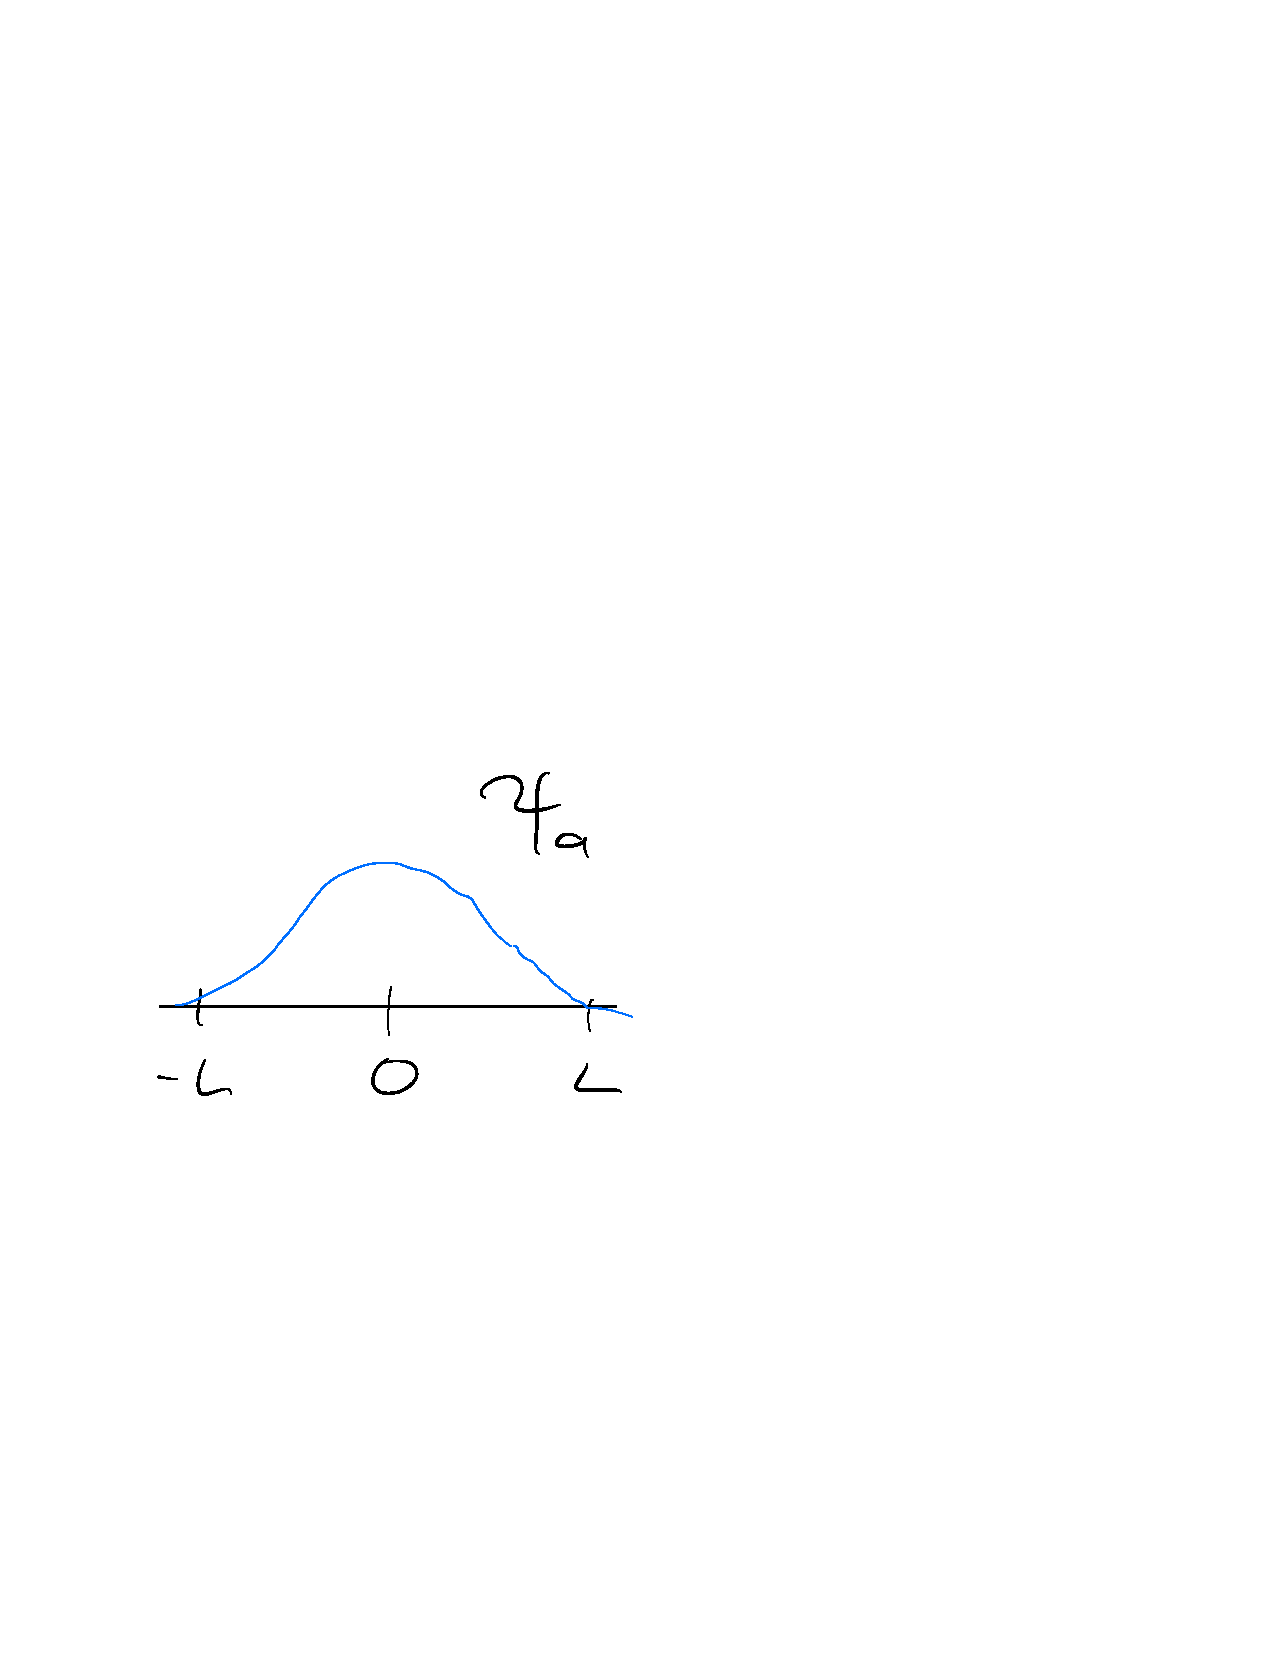
\includegraphics[width=0.3\textwidth]{./psia.pdf}
\hspace{0.3in}
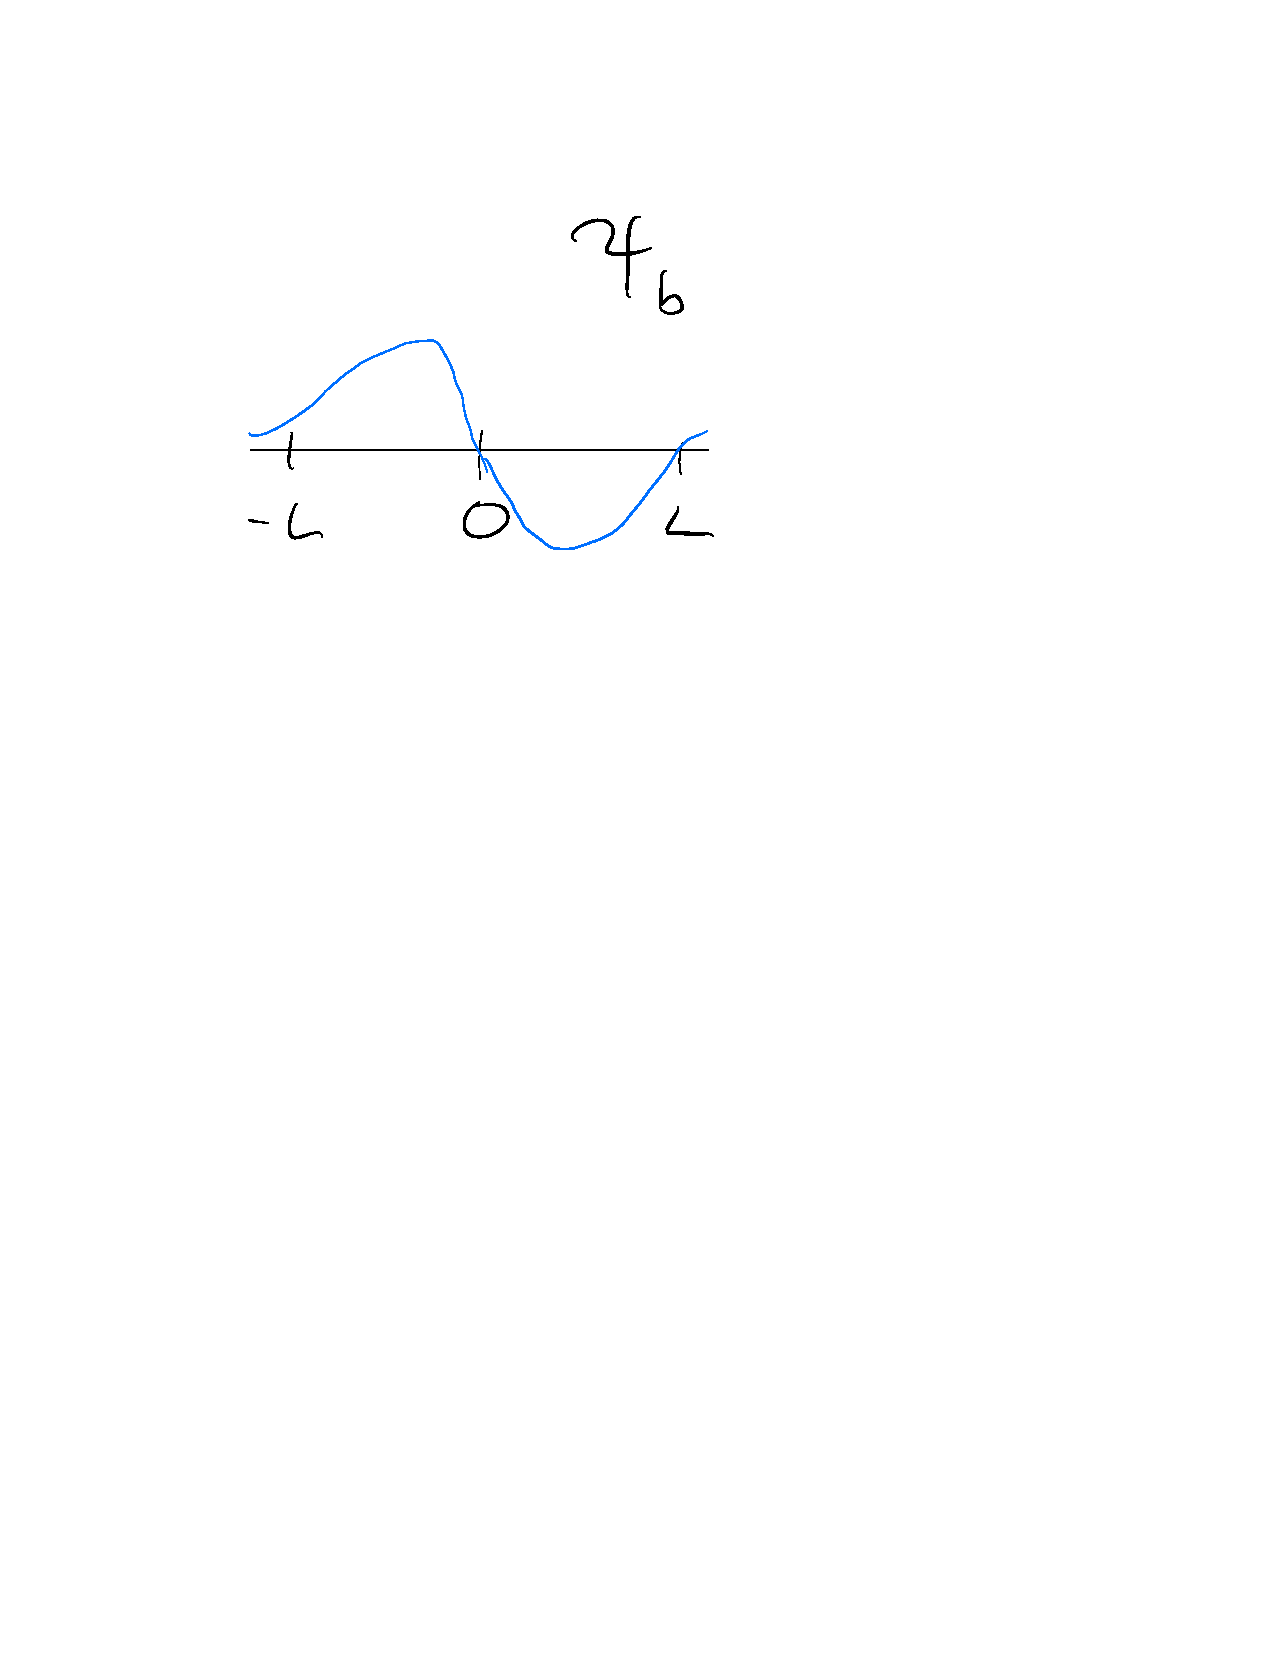
\includegraphics[width=0.3\textwidth]{./psib.pdf}
\end{center}


Which wave function has the large expectation value for $<x>$ ?
Which wave function has the large expectation value for $<p>$ ?
Explain.
}
\item[(b)]{
Suppose you start with a particle with wave-function $\psi_b$ and repeatedly measured it's position.
Sketch the expected distribution of position measurements. 
Discuss.
}
\item[(c)]{
Suppose you start with an ensamble of different particles, each with wave-function $\psi_b$, and measure each of their positions.
Sketch the expected distribution of position measurements. 
Discuss.
}
\end{itemize}

\vspace*{0.4in}

\textbf{3) Integration By Parts. } \hfill \textit{(15 points)}\\

Use integration by parts to show that
\begin{equation*}
 <p> = -i\hbar \int \psi^* \frac{\partial \psi}{\partial x} dx
\end{equation*}

\clearpage


\textbf{4) Relation of Quantum Mechanics to Classical Physics   } \hfill \textit{(40 points)}\\ 
\begin{itemize}
\item[(a)]{ 
Show that :
\begin{equation}
m \frac{d^2 \langle x \rangle}{dt^2} = \langle - \frac{\partial V}{\partial x} \rangle.
\end{equation}
This tells us that the expectation values obey the \textit{classical}  laws of physics.
}
\item[(b)] {
In classical physics adding a constant $V_0$ to the potential energy doesn't change anything.
What happens in Quantum Mechanics? \\ \\
Show that the wave function picks up a time-dependent phase factor. eg: $\psi \rightarrow e^{-iV_0 t/\hbar}\psi$ when $V \rightarrow V + V_0$.  \\ \\
What effect does this have on the expectation value of dynamic variables ?
}
\item[(c)] {
The purpose of this problem is to build your intuition as to which systems have to be treated quantum mechanically, and which can safely be described classically. \\
 
Quantum mechanics is relevant when the de Broglie wavelength of a particle is greater than the characteristic size of the system (d). 
In thermal equilibrium at temperature T, the average kinetic energy of a particle is 
\begin{equation}
\frac{p^2}{2m} = \frac{3}{2} k_B T
\end{equation}
where $k_B$ is the Boltzmann's constant. 

\textbf{Solids:} The lattice spacing of a solid is $d\sim0.3$ nm. 
Find the temperature below which the free \textit{electrons} in a solid are quantum mechanical. 
Below what temperature are the \textit{nuclei} in a solid quantum mechanical ?
(Use sodium as a typical case)


\textbf{Gases:} For what temperatures are the atoms in an ideal gas at pressure P quantum mechanical? 
(\textit{Hint:} Use teh ideal gas law to deduce d.
Put in the numbers for helium at atmospheric pressure.
Is hydrogen in outer space ($d\sim cm$ and $T \sim 3 K$) quantum mechanical? 
}
\item[(d)] {
In classical physics the energy is a real number. 
Show that for normalizable wave functions the E must also be real. 
(\textit{Hint:} show that $\frac{d}{dt}\int |\psi|^2 dx = 0$ only if E is real.)
}
\end{itemize}



  

\end{document}
